
% JuliaCon proceedings template
\documentclass{juliacon}
\setcounter{page}{1}

\usepackage{amsmath}
\usepackage{siunitx}
\usepackage{mathtools}
\usepackage{graphicx}
%\usepackage{caption} %For subfigures
%\usepackage{subcaption} %For subfigures

\begin{document}

% **************GENERATED FILE, DO NOT EDIT**************

\title{SyntheticEddyMethod.jl}

\author[(1,2,3)]{Carlo Brunelli}
\author[1]{Bart Janssens}
\author[2]{Georg May}
\author[3]{Mark Runacres}
\affil[1]{Mechanical Engineering Department, Royal Military Academy, Belgium}
\affil[2]{Aeronautics and Aerospace Department, von Karman Institute for Fluid Dynamics, Belgium}
\affil[3]{Engineering Technology Thermodynamics and Fluid Mechanics Group, VUB, Belgium}

\keywords{Julia, Turbulence, Eddy, Inlet Condtions}

\hypersetup{
pdftitle = {SyntheticEddyMethod.jl},
pdfsubject = {JuliaCon 2022 Proceedings},
pdfauthor = {Carlo Brunelli, Bart Janssens, Georg May, Mark Runacres},
pdfkeywords = {Julia, Turbulence, Eddy, Inlet Condtions},
}



\maketitle

\begin{abstract}
This study presents the implementation of a Synthetic Eddy Method (SEM) in the Julia programming language and its validation through statistical analysis. SEM is a widely used technique for simulating turbulent fluid flows, and its efficient implementation in Julia makes it an attractive tool for researchers and engineers. \texttt{SyntheticEddyMethod.jl} aims to be in fluid dynamics simulations for creating suitable inlet conditions. Turbulence is frequently examined using incompressible models. This has led to the development of the Divergence-Free Synthetic Eddy Method (DFSEM), which enforces the constraint of respecting the divergence-free condition introduced by the continuity equation for the synthetic eddies.
We first describe the implementation of SEM and DFSEM in Julia, highlighting its advantages over other programming languages. We then validate the accuracy of the method through statistical analysis of simulated data. Specifically, we compute the statistical moments and probability density functions of velocity fluctuations generated by SEM. The results show good agreement between the values and the expected results, validating the accuracy of the SEM implementation in Julia. Overall, this study demonstrates the utility of Julia as a programming language for simulating turbulent flows using SEM and provides a framework for future studies using this technique.
\end{abstract}

\section{Introduction}
In the past decades, large eddy simulations (LES) and ---where computationally possible--- direct numerical simulations have been widely used for simulating complex flows such as separation and turbulence. In order to increase the accuracy of the results, the generation of realistic inflow data for LES is a crucial problem. In fact, the inflow boundary condition is also turbulent and unsteady. Many methods can be found in the literature regarding inflow generators and they can be grouped into three families: precursor simulation or databases, recycling methods and synthetic turbulence, \cite{Pamies}. Synthetic Eddy Methods (SEM), first introduced by Jarrin et al. \cite{Jarrin2006}, are a family of techniques to generate realistic inflow data for LES simulation. Compared with precursor simulation and recycling methods, the synthetic methods in general offer a more practical and relatively efficient approach to generating inflow turbulence and are therefore widely adopted. The widespread use of this family of methods is driven by the constant research to increase the accuracy of the fluid simulations. Another significant aspect is that these methods can also be employed for reducing the time required by the fluid to be statistically stable. Non-realistic initial conditions, such as white noise, might not be the best choice. It creates high velocity gradients in the fluid, which are quickly dissipated and, in the case of the turbulent channel study, it can even lead to a re-laminarization of the flow, \cite{LUND1998233}. The inflow data does not have any temporal or spatial correlation. 
A new methodology, named Divergence Free SEM (DFSEM), has been recently introduced by \cite{Poletto2013} which is able to apply also the divergence-free constraint for incompressible flows. The  improved  method,  when  used  to  provide suitable inlet  conditions, claims to reduce  near-inlet  pressure  fluctuations and also to reduce the development length.


\section{Synthetic Eddy Method foundations}
The Synthetic eddy method approach has been introduced by Jarrin et al.\cite{Jarrin2006}.
The first goal is to generate a turbulent velocity conforming to the formula \eqref{sem:u}.
\begin{equation}
    \Vec{u}(\Vec{x},t) = \Vec{U}(\Vec{x},t) +  \Vec{u'}(\Vec{x},t)
    \label{sem:u}
\end{equation}
where $\Vec{U}(\Vec{x},t)$ and $\Vec{u'}(\Vec{x},t)$ are respectively the mean and the fluctuating velocity at location $\Vec{x}$ at the instant $t$. 
The method relies upon the representation of turbulent spots or eddies by shape function $f$. In one dimension, the shape function needs to have compact support over [-1,1] and satisfy the normalization condition \eqref{sem:normalization}.
\begin{equation}
    \int_{-1}^{1} f^2(x)dx = 1
    \label{sem:normalization}
\end{equation}

Many different choices of shape functions are available, tent function \ref{sem:tent}, step function  \ref{sem:step}, truncated gaussian \ref{sem:gaus}  where $C=1.301$ is a coefficient that allows the shape function to satisfy the normalization coefficient.
\begin{equation}
f = 
\begin{cases}
  \sqrt{\dfrac{3}{2}}(1-|x|) & |x|\leq 1 \\
  0 & |x|>1
\end{cases}
\label{sem:tent}
\end{equation}

\begin{equation}
f = 
\begin{cases}
  \dfrac{1}{\sqrt{2}} & |x|\leq 1 \\
  0 & |x|>1
\end{cases}
\label{sem:step}
\end{equation}


\begin{equation}
f = 
\begin{cases}
  C e^{-9/x^2} & |x|\leq 1 \\
  0 & |x|>1
\end{cases}
\label{sem:gaus}
\end{equation}

\begin{figure}[h]
     \centering
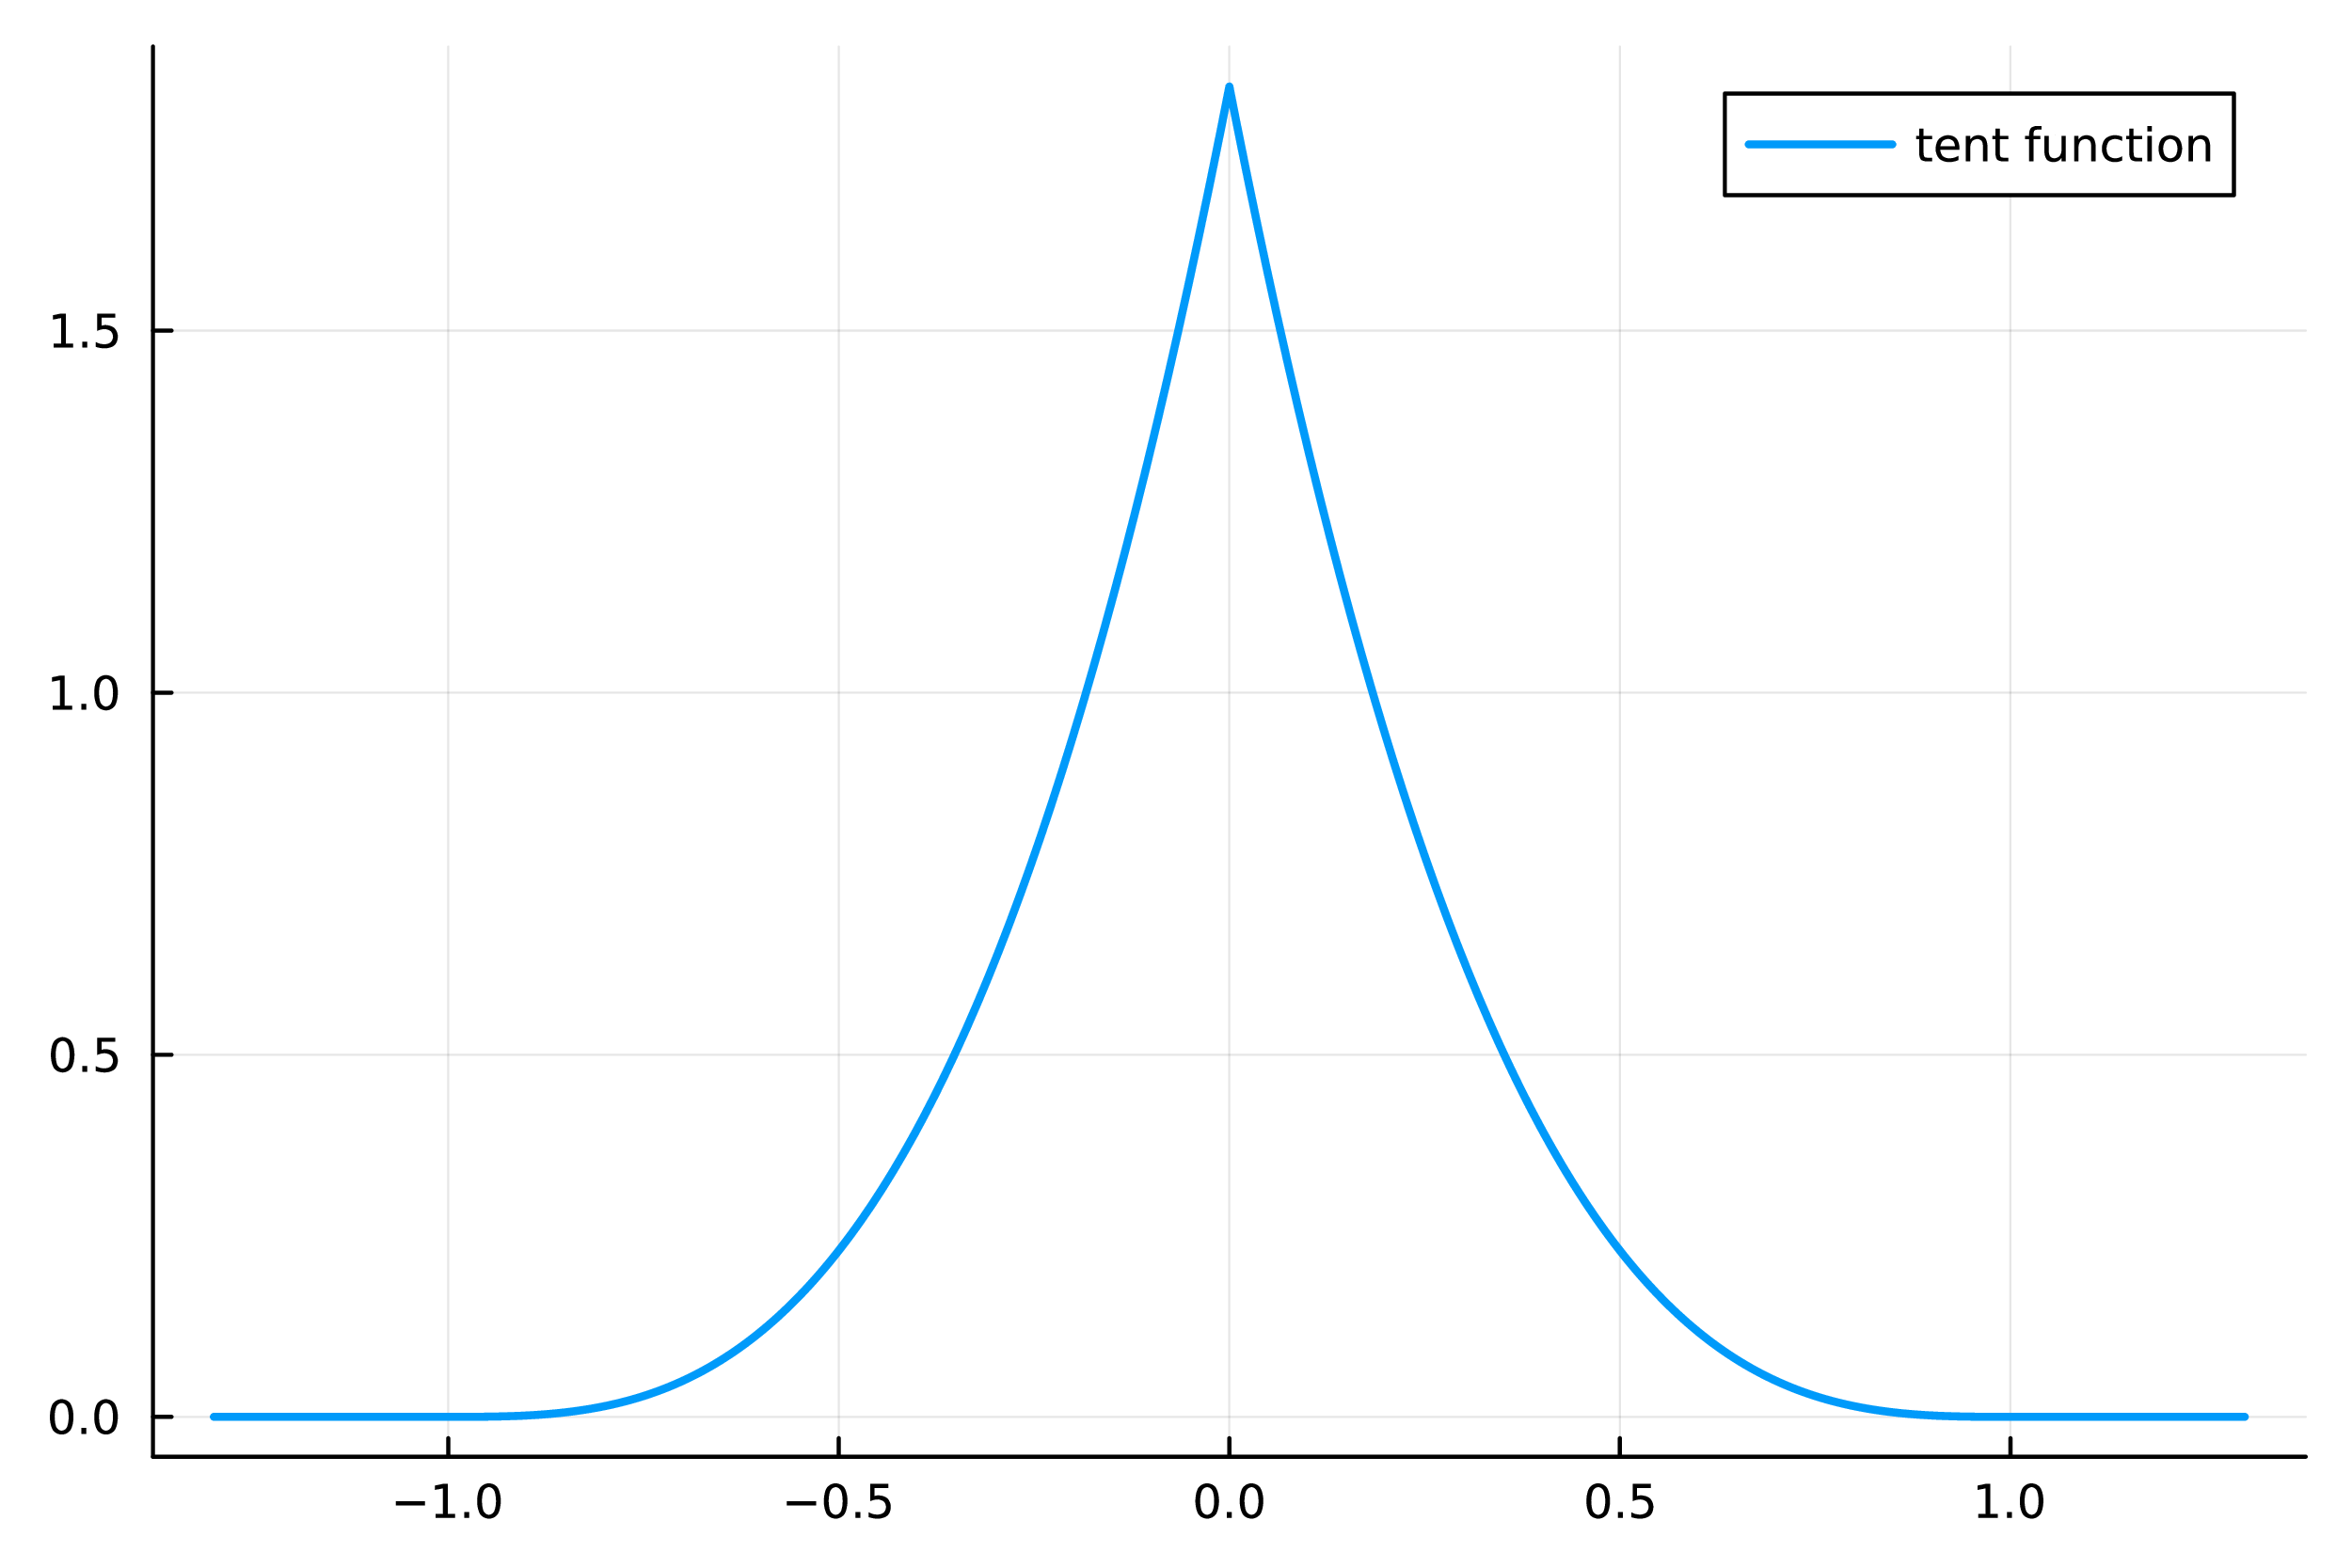
\includegraphics[width=0.45\textwidth]{Images/shape/tent_fun.png}
         \caption{Tent function}          
         \label{figsem:tent_fun}
\end{figure}

\begin{figure}[h]
     \centering
         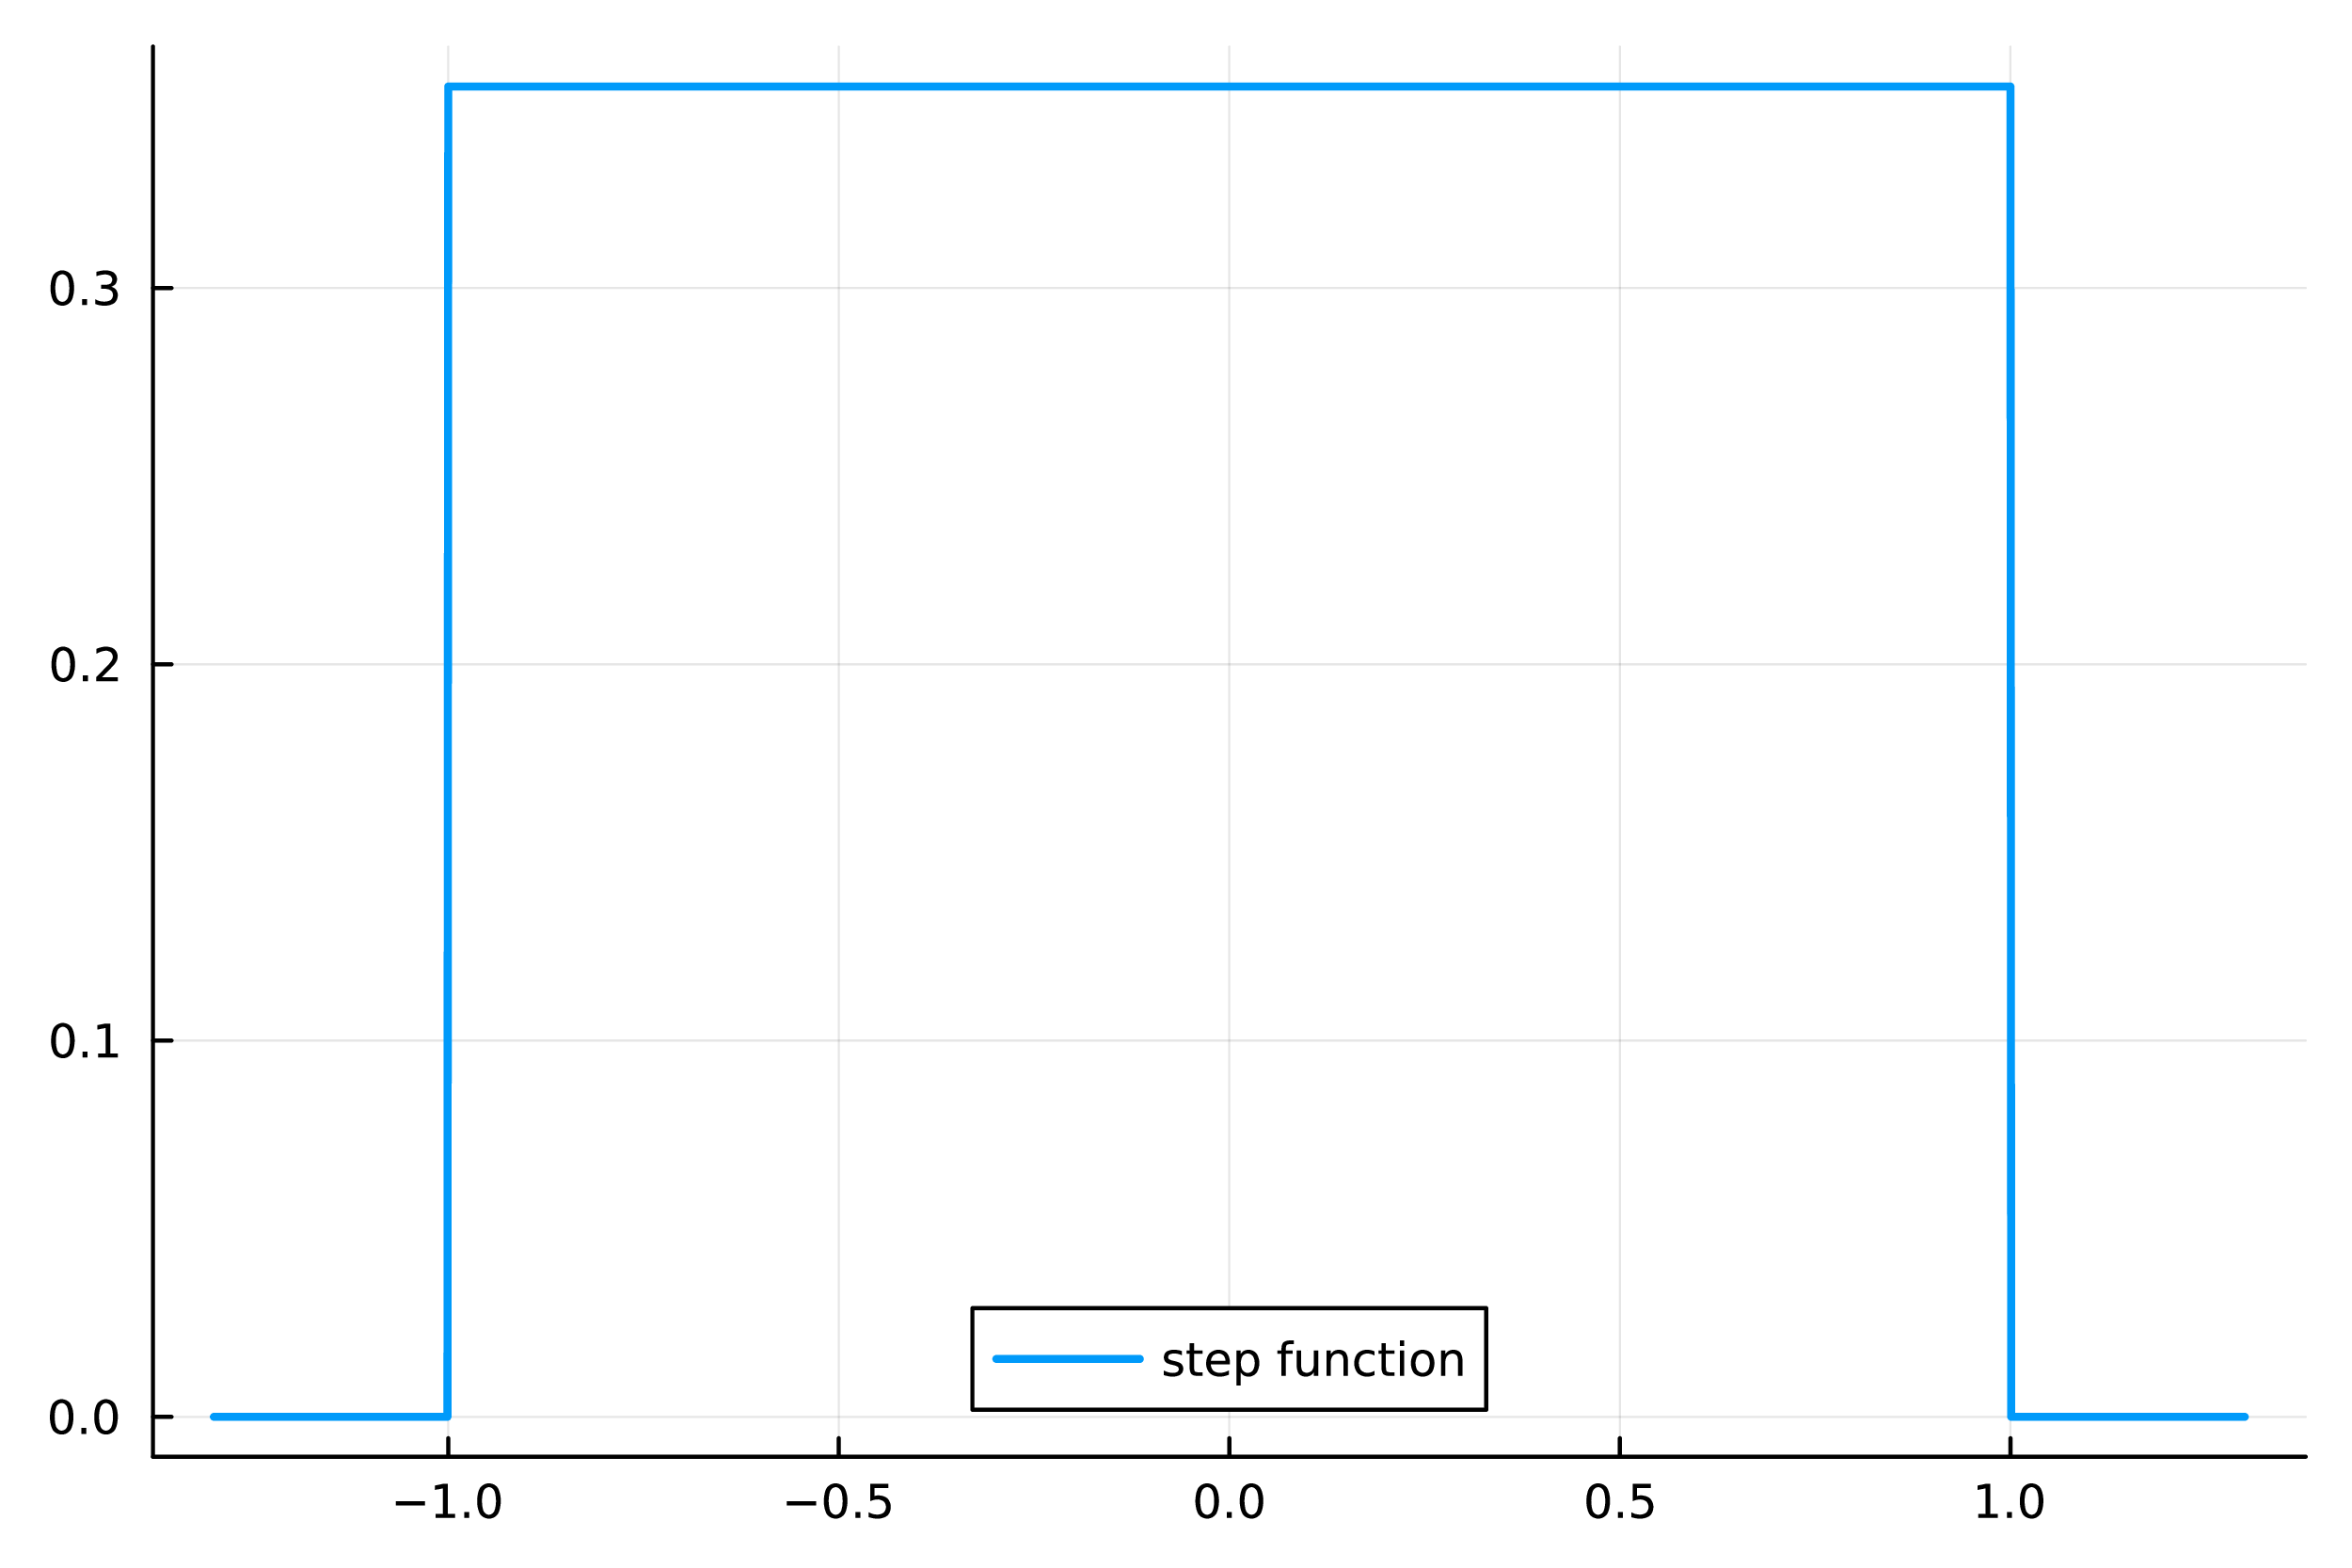
\includegraphics[width=0.45\textwidth]{Images/shape/step_fun.png}
         \caption{Step function}
            \label{figsem:step_fun}
\end{figure}

\begin{figure}[h]
     \centering
         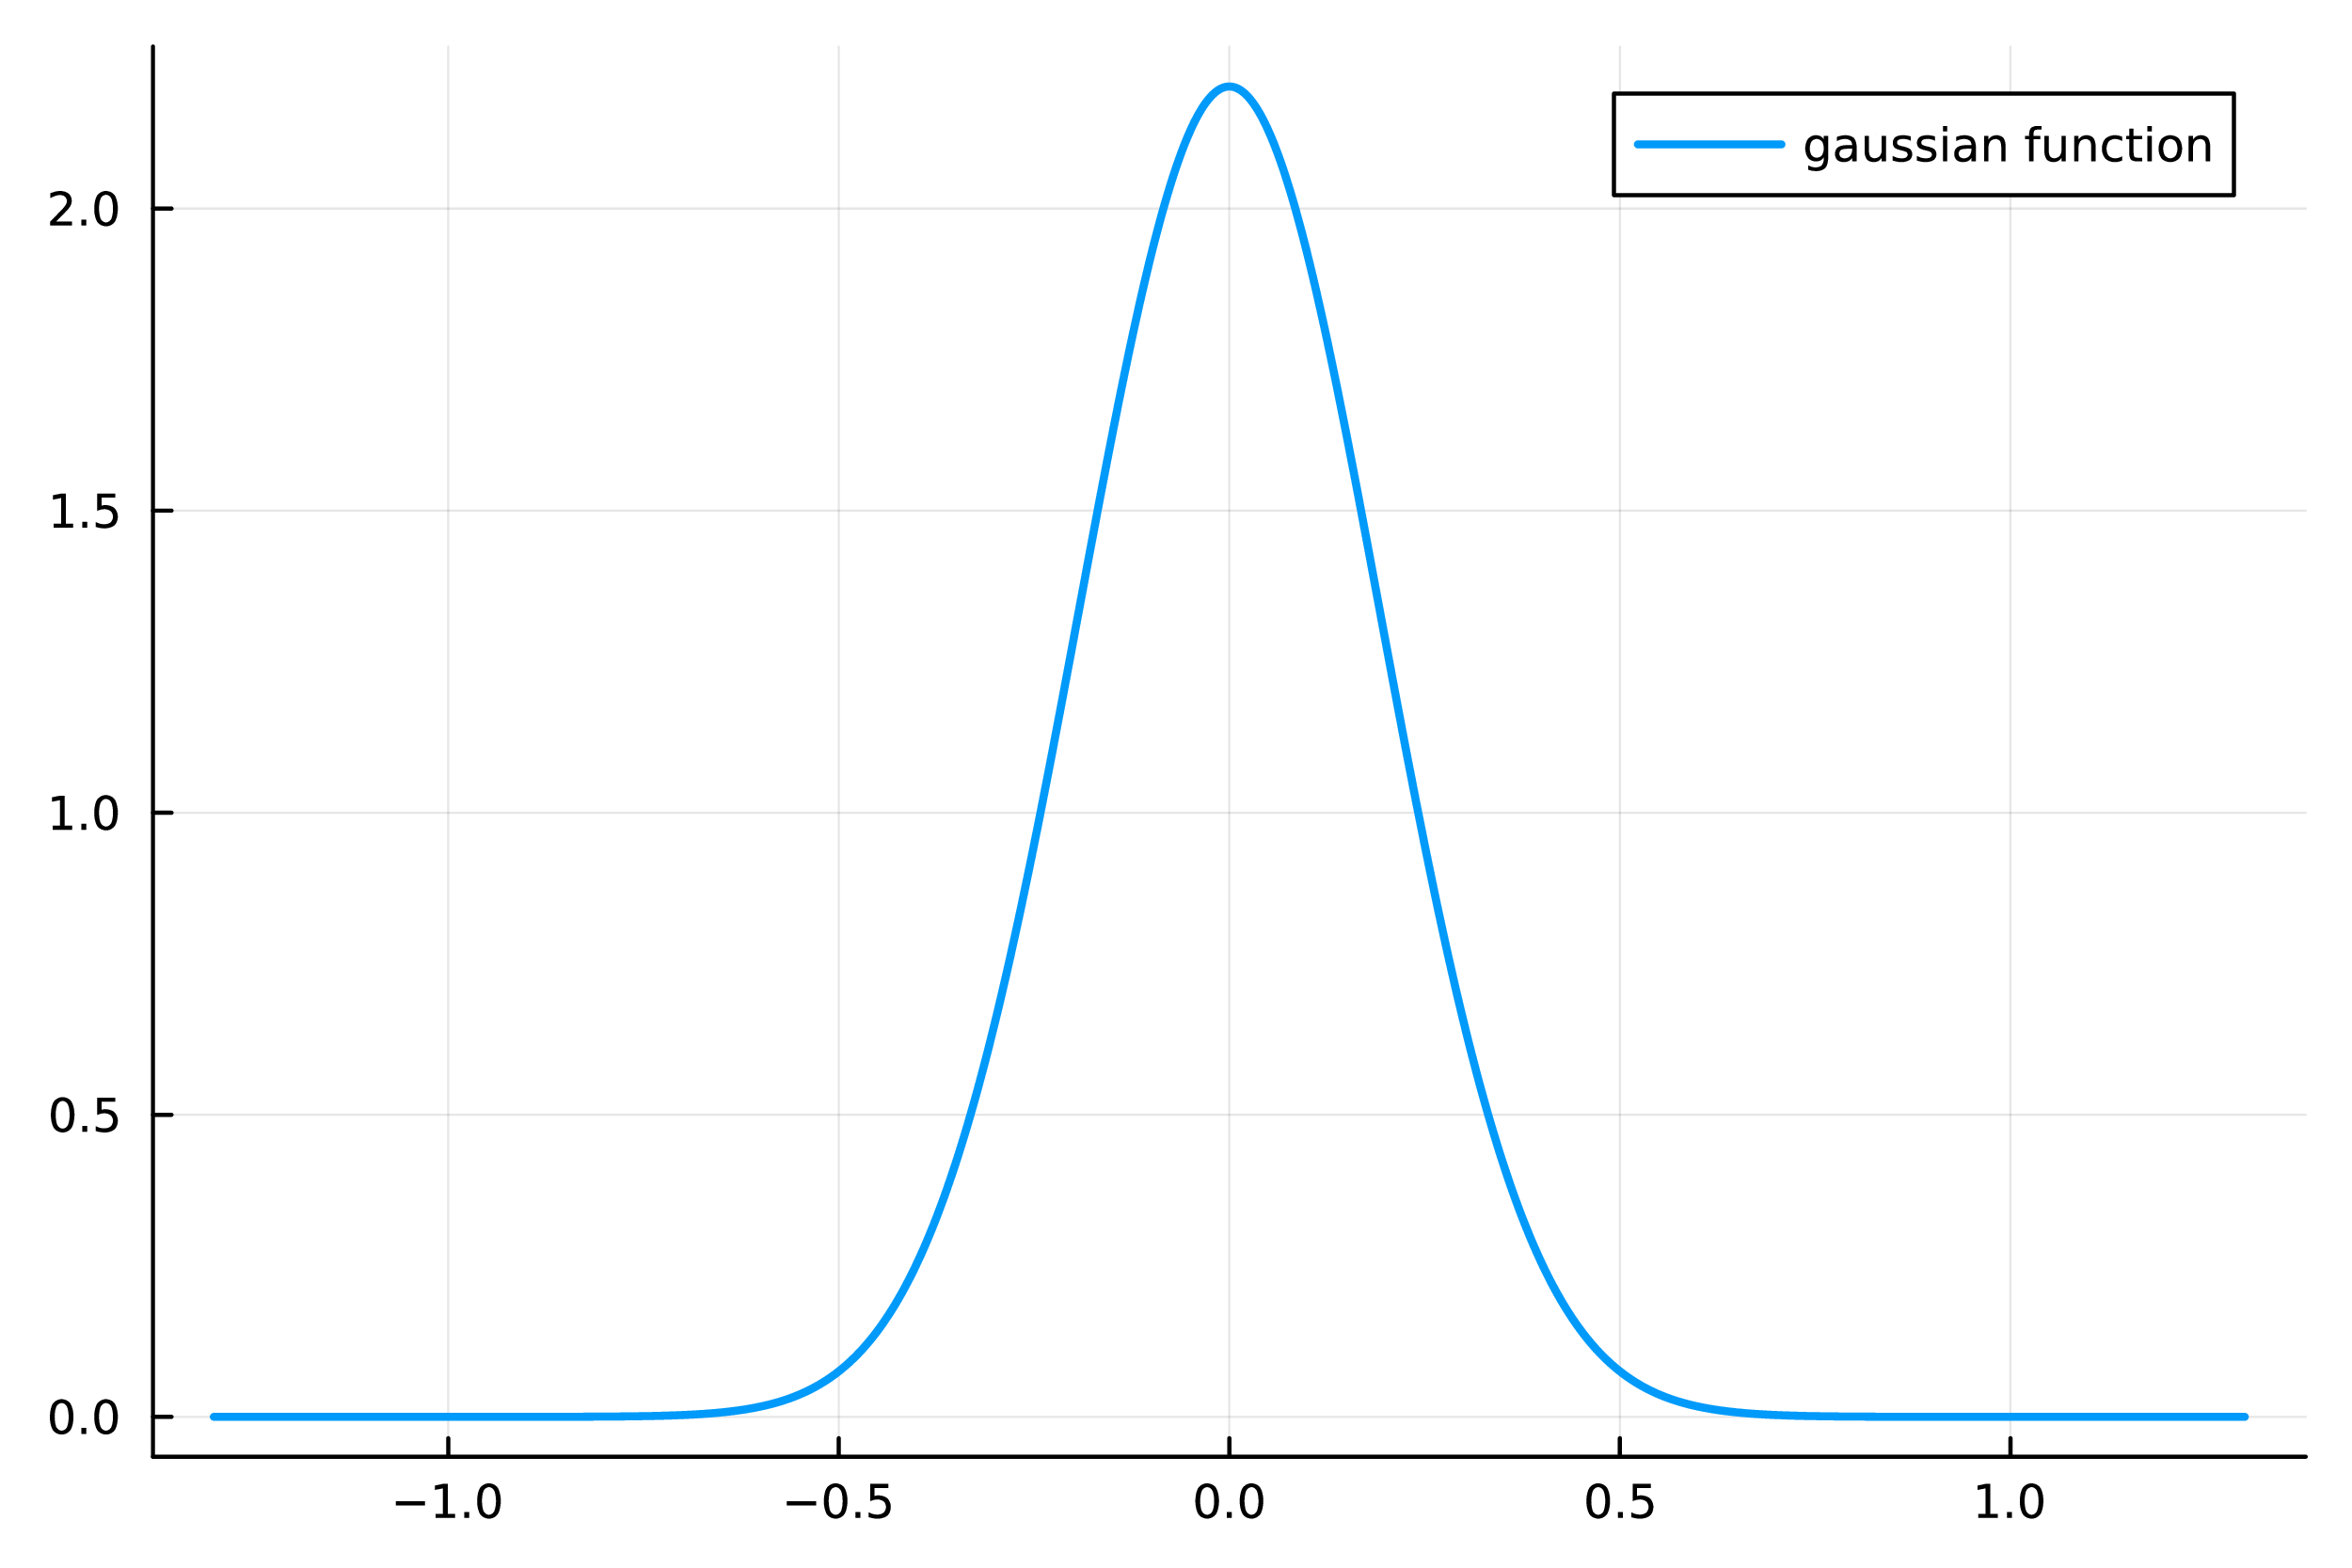
\includegraphics[width=0.45\textwidth]{Images/shape/trun_gauss_fun.png}
         \caption{Truncated Gauss function}
            \label{figsem:gauss_fun}
\end{figure}




A fundamental parameter for defining eddies is $\sigma$, which represents the dimension. In the case of isotropic turbulence $\sigma$ is the same for all three directions. A common choice for  $\sigma$ is $\sigma = 2\Delta z$ where $\Delta z$ is the mesh length in $z$ direction.

The inflow region, usually a plane, is a set of points where synthetic turbulence needs to be generated and evaluated. This set of points $S = {x_1, x_2, x_3 ...}$ needs to be inside the so-called \textbf{virtual box} $B$ where the eddies are created which is a three-dimensional box-shaped fictitious region.
$$B = \{(x_1,x_2,x_3) \in 	\mathbb{R}^3: x_{i,min}<x<x_{i,max} \}$$
where $\forall x \in S$
$$x_{i,min} = min(x_i-\sigma_i(x)) \text{ and } x_{i,max} = max(x_i+\sigma_i(x)) $$
It means that the virtual box is slightly larger than the strictly necessary to ensure better coverage also of the boundary points of the inlet plane.
The number of eddies, $N$, inside the virtual box is also crucial. In order to provide sufficient statistical coverage, Pamies \cite{Pamies} suggests the estimation of N using the formula \eqref{sem:num} where $S_p$ is the surface transverse to the virtual box and $S_s$ the transverse surface of the shape function (for isotropic case $\sigma\cdot\sigma$), \ref{figsem:Vbox_SsSp}. It provides accurate results for a planar inlet surface, while it needs to be adjusted for curved inlet planes.
\begin{equation}
    N = \dfrac{S_p}{S_s}
    \label{sem:num}
\end{equation}

\begin{figure}[h]
     \centering
         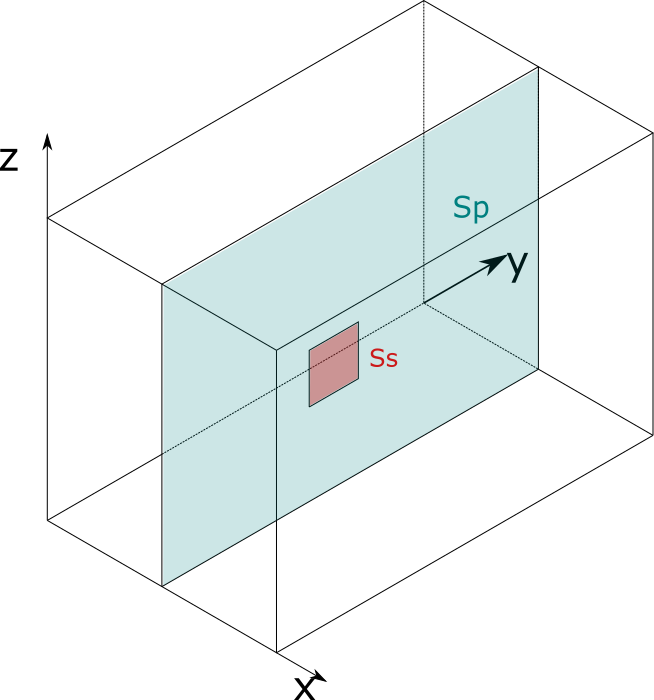
\includegraphics[width=0.45\textwidth]{Images/virtual_box.png}
         \caption{Virtual Box and Sp and Ss from equation \eqref{sem:num}}
            \label{figsem:Vbox_SsSp}
\end{figure}


Finally, the equation for the component $i$ of the velocity is \eqref{sem:ui}.
\begin{equation}
u_i(\boldsymbol{x})=U_i(\boldsymbol{x})+\frac{1}{\sqrt{N}} \sum_{k=1}^N a_{i j} \epsilon_j^k f_{\sigma(\boldsymbol{x})}\left(\boldsymbol{x}-\boldsymbol{x}^k\right)
\label{sem:ui}
\end{equation}
where $\Vec{x}$ represents the coordinates of the computational points and $x^k$ the k-eddy's centre coordinate. The $\epsilon_j^k$ factor is called intensity, and it can be -1 or 1. The idea is that spots are located randomly over the virtual box, and they can have a positive or negative intensity. This is coherent with the fact that fluctuations can increase or reduce the local velocity. The $a_{i,j}$ terms come from the Cholesky decomposition \eqref{sem:chol} of a prescribed Reynolds stress tensor which is usually known a priori from previous experiments, DNS or RANS calculations.
\begin{equation}
\left(\begin{array}{ccc}
\sqrt{R_{11}} & 0 & 0 \\
R_{21} / a_{11} & \sqrt{R_{22}-a_{21}^2} & 0 \\
R_{31} / a_{11} & \left(R_{32}-a_{21} a_{31}\right) / a_{22} & \sqrt{R_{33}-a_{31}^2-a_{32}^2}
\end{array}\right)
\label{sem:chol}
\end{equation}

\begin{equation}
\begin{multlined}
f_{\sigma(\boldsymbol{x})}\left(\boldsymbol{x}-\boldsymbol{x}^k\right)= \\
=\sqrt{\frac{V_B}{\sigma_1 \sigma_2 \sigma_3}} f\left(\frac{x_1-x_1^k}{\sigma_1}\right) f\left(\frac{x_2-x_2^k}{\sigma_2}\right) f\left(\frac{x_3-x_3^k}{\sigma_3}\right)
\end{multlined}
\label{sem:fsigma}
\end{equation}

Equation \eqref{sem:fsigma} presents the generic case where there are different $\sigma$ in different directions, and $V_B$ is the virtual box volume.

In the formulas \eqref{sem:ui} and \eqref{sem:u} you may notice that the dependence of time has been removed. The eddies are convected through the virtual box with the convective velocity $U_0$ using Taylor’s frozen  turbulence hypothesis \ref{sem:convect}. Once the eddy's centre coordinate reaches the end of the virtual box it is re-generated at the virtual box entrance.
\begin{equation}
    x_i(t+dt)=x_i(t)+U_0 dt
    \label{sem:convect}
\end{equation}
In the virtual box, there is no dissipation, it is not physical and eddies are just convected in the $x$ direction.

\section{Divergence Free Synthetic Eddy Method extension}
The DFSEM is an evolution of the SEM that addresses this issue by adding the constraint of ensuring that the synthetic eddies do not produce any divergence in the flow field. We are following the notation and procedure explained in \cite{Polettoreport}. The DFSEM guarantees continuity by utilizing the SEM technique on the vorticity field and then converting it to a corresponding velocity field. This involves applying \eqref{sem:ui} to generate perturbations in the vorticity field and relating the curl of the vorticity to the velocity Laplacian, \eqref{sem:vort}.

\begin{equation}
    \nabla \times \Vec{\omega}'  = \nabla(\nabla\cdot \Vec{u'}) - \nabla ^2 \Vec{u'}
    \label{sem:vort}
\end{equation}

The first term of the equation \eqref{sem:vort} is zero due to the continuity condition. Using the Biot-Savart kernel is possible to retrieve the velocity field, \eqref{sem:vort2}, where $q_\sigma$ is a suitable shape function and $\Vec{\alpha}$ depends on the eddy intensity and the prescribed Reynolds Stress tensor.

\begin{equation}
\Vec{u'}(\Vec{x}) =  \sqrt{\dfrac{1}{N}} \sum_{k=1}^N \dfrac{q_\sigma(|y|}{|y|^3} \times \Vec{\alpha_k}
    \label{sem:vort2}
\end{equation}

\begin{figure}[h]
     \centering
         \includegraphics[width=0.45\textwidth]{Images/shape/DFSEM_fun.pdf}
         \caption{DFSEM function, \eqref{sem:dfsemfun}}
            \label{figsem:dfsem_fun}
\end{figure}

The shape function chosen to be implemented is \eqref{sem:dfsemfun}, where $d_k$ is the normalized distance between one point and the $k-th$ eddy, \eqref{sem:dk}.
\begin{equation}
q_\sigma (d_k) = 
\begin{cases}
  \sqrt{\dfrac{16V_B}{15\pi \sigma^3}}(sin(\pi d_k))^2\cdot d_k & |d_k|\leq 1 \\
  0 & |d_k|>1
\end{cases}
\label{sem:dfsemfun}
\end{equation}
$$
\Vec{r_k} = \begin{bmatrix}x-x_k\\y-y_k\\z-z_k\end{bmatrix}
$$
\begin{equation}
d_k = \dfrac{|r_k|}{\sigma}
\label{sem:dk}
\end{equation}


In order to obtain the $\Vec{\alpha}$ parameter the equation \eqref{sem:vort2} is averaged. Then, to get the desired Reynolds stress tensor is convenient to work in the principal axes. The coefficients $\alpha_{i,k}$ from equation \eqref{sem:vort2} can be obtained with \eqref{sem:alpha}, where $k'$ is the turbulent kinetic energy and $\lambda_i$ is the corresponding eigenvalue. Note, the turbulent kinetic energy is written as $k'$ and not $k$ for distinguishing it from the index.

\begin{equation}
    \alpha_{i,k} = \sqrt{2(k'-\lambda_i)}\epsilon_{i,k}
    \label{sem:alpha}
\end{equation}

However, equation \eqref{sem:alpha} is valid in principal (or local, superscript $L$) axes, it has to be rotated back to the original (or global, superscript $G$) axes. The final fluctuations equation that respects the divergence-free conditions is \eqref{sem:dfsemui}.


\begin{equation}
\Vec{u'}(\boldsymbol{x})=\frac{1}{\sqrt{N}} \sum_{k=1}^N \dfrac{q_\sigma(d_k)}{d_k^3} \dfrac{\Vec{r_k}}{\sigma}\times[R_L^G(\sqrt{(2(k'-\lambda_i)}\epsilon_k]
\label{sem:dfsemui}
\end{equation}


\section{Implementation and usage}
The Julia implementation closely adheres to the mathematical framework presented in the previous section, minimizing the user's effort required for parameter setup. The first step involves specifying the virtual box dimensions while ensuring the inflow simulation plane is fully contained within the box. The parameter $\sigma$ is fundamental, it represents the eddies dimension. Additionally, the shape function must be set, with the tent function being the default option. The user can manually set the Reynolds stress tensor or provide a database with pre-existing values. By default, the code employs a simple diagonal tensor that is calculated based on the specified turbulence intensity and mean flow velocity. 
A Cholesky decomposition for the 3x3 Reynolds stress tensor is also encoded.

In the implementation of the DFSEM, especially in the computation of the $\alpha_k$ parameter the \texttt{LinearAlgebra.jl} package has been extensively used. For working in principal axes and passing from local to global reference systems the computation of eigenvalues and eigenvectors comes in handy. For computing the turbulent kinetic energy $k'$ the trace of the Reynolds stress is computed, and divided by 2, \eqref{sem:tke}.
\begin{equation}
    k' = \dfrac{1}{2} (<u_1'u_1'> + <u_2'u_2'> + <u_3'u_3'>)
    \label{sem:tke}
\end{equation}
Mathematical condition of existence arises from equation \eqref{sem:alpha}, $k' > max(\lambda_i)$. It means that not all the anisotropy conditions can be properly reproduced. 


In contrast to other programming languages, Julia achieves the same objective with significantly less code. For instance, the code \cite{Oh2019}, developed in FORTRAN and used as an initial source of inspiration, is less concise and expressive, less user-friendly, and more challenging for others to contribute to. In this Julia code, users can effortlessly implement a new shape function by examining how the existing ones are implemented.

\subsection{Eddy storage}
An array containing all the eddies information is created. Each eddy is a structure that stores the eddy identification number, its center position and dimensions along the three axes ($\sigma_x, \sigma_y, \sigma_z$). Although the eddies' dimensions may initially appear as redundant storage of information, it enables future versions to feature eddies with varying dimensions in different areas of the domain. This property has the potential to improve simulations of turbulent channels.
One of the advantages of this implementation is that the virtual box has almost and infinite precision, not related to the mesh discretization in the LES simulation. The values of the fluctuation in velocity can be computed in any point of the virtual box.
The code can be conveniently integrated with a particular fluid dynamics code. Alternatively, it can be pre-run to store velocity values, which can then be loaded during the fluid simulation run.

\section{Tests and statistical assessment}
The objective of the tests is to confirm that the fluctuations generated by the SEM are more realistic than those that can be easily produced by a random signal. Additionally, the statistical characteristics of the turbulent fluctuations produced will be verified. The tests are made taking into account a flat plane of dimensions YZ: $[0,5]\times[0,5]$ and $\sigma=0.1$. The virtual box is then $[-0.1,0.1]\times[-0.1,5.1]\times[-0.1,5.1]$. The temporal velocity fluctuations of the point at the centre of the domain are analyzed. The convective velocity in the $X$ direction is set at $U_0=1m/s$ and the time step is $0.01s$, so each eddy takes 10 time-steps to pass through the full domain. The tent function is adopted as a shape function.

\subsection{Standard deviation and autocorrelation analysis}
In this section, the goal is to confirm that the root-mean-square of the generated fluctuations is close to the prescribed turbulence intensity. 50 independent tests have been launched for $\num{100000}$ time steps each. At the end of each, the root-mean-square of each velocity component has been computed. 
Figure \ref{figsem:mean} shows how the mean value of velocity is converging during the $\num{100000}$ time steps. It requires a significant time to have a fully converged mean velocity, due to the relatively high turbulence intensity value. In figure \ref{figsem:fluct} the density function of the computed fluctuation values is reported. The root-mean-square of the 3 components of velocity has been used together, adopting the hypothesis of independence of fluctuations in different directions. The mean value is $2\%$ less than the expected one, with a standard deviation of $\sigma=0.003$. 
The plots \ref{figsem:autocorr} shows the autocorrelation of the fluctuations in a single run for the 3 velocity components. The 3 autocorrelation curves are almost overlapping. In this case, the convective velocity is $U_0 = 1m/s$ and the time step $dt=0.01s$. It means that $0.1s$ corresponds to a length of $0.1m$, which is the eddies size. It is the same order of magnitude of the integral time scale $T\approx 0.072s$, which has been computed accordingly to the formula \ref{sem:integraltimescale}.

\begin{equation}
T = \int_0^\infty r(\tau)d\tau
    \label{sem:integraltimescale}
\end{equation}



\begin{figure}[h]
     \centering
     \centerline{\includegraphics[width=0.45\textwidth]{Images/Statistics/SEM_Fluctuations.pdf}}
         \caption{Root-mean-square of the fluctuations}          
         \label{figsem:fluct}
\end{figure}


\begin{figure}[h]
     \centering
         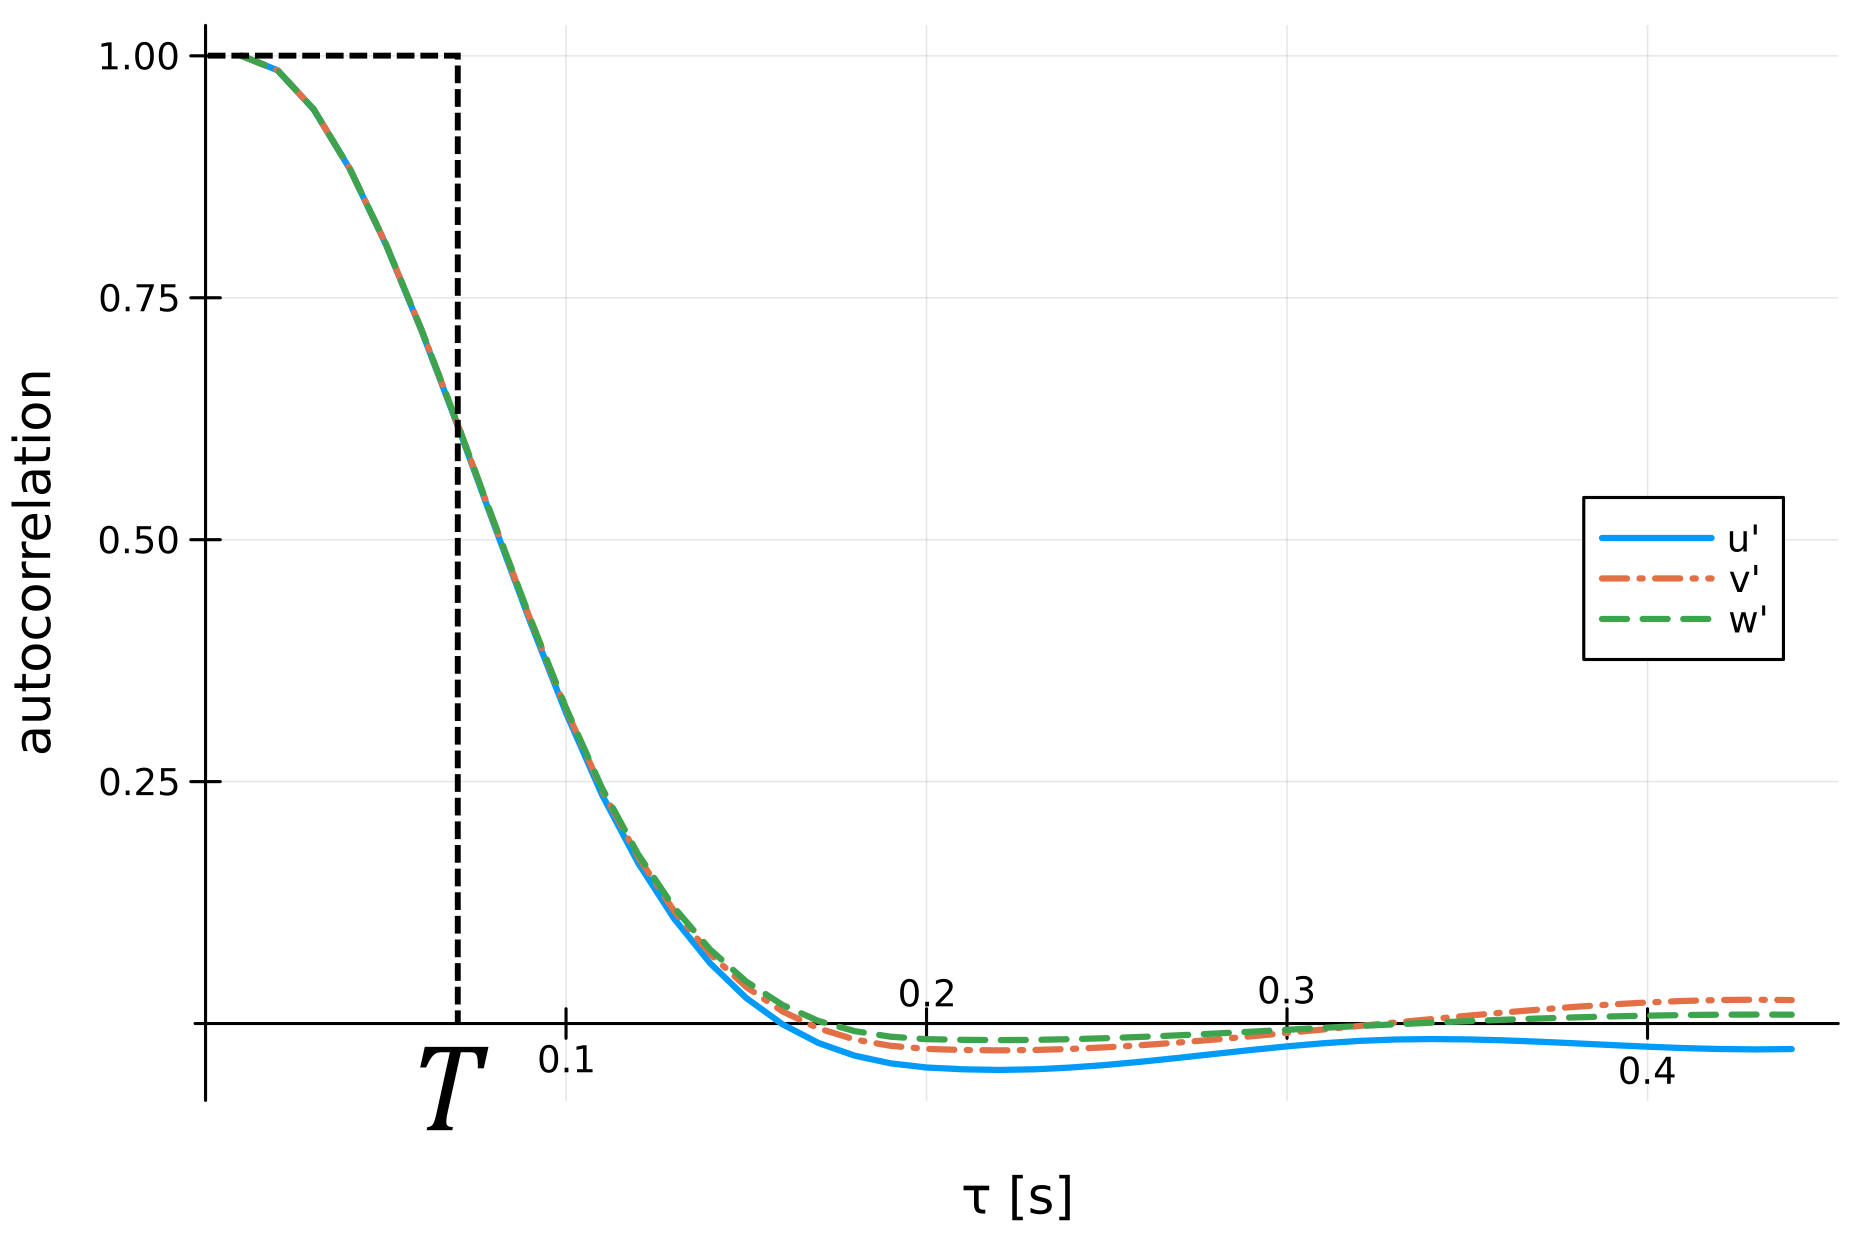
\includegraphics[width=0.45\textwidth]{Images/Statistics/autocorr.png}
         \caption{Autocorrelation with time delay for the point at the centre of the inlet plane}
            \label{figsem:autocorr}
\end{figure}


\begin{figure}[h]
     \centering
         \includegraphics[width=0.45\textwidth]{Images/Statistics/SEM_mean.pdf}
         \caption{Convergence of the fluctuations towards the  zero mean value within $\num{20000}$ time-step}
            \label{figsem:mean}
\end{figure}

 



\subsection{Power Spectral analysis}
The primary objective of this study is to examine and validate the capability of the Synthetic Eddy Method (SEM) to generate a signal that is consistent with turbulence. To achieve this objective, the spectral curves produced by the SEM have been analyzed in the inertial subrange. The spectral curves generated by the SEM have been found to adhere relatively closely to the $k^{-5/3}$ power law trend, which is indicative of turbulence. This consistency between the SEM-generated spectral curves and the $k^{-5/3}$ trend is a key indicator of the ability of the SEM to produce signals that are similar to actual turbulence.

In contrast, when random signals are generated, there is equal energy distributed among all wave numbers. This results in a flatter spectral curve that does not follow the $k^{-5/3}$ trend. Therefore, the spectral curves generated by the SEM are a more realistic representation of turbulence than those produced by random signals.

Moreover, increasing the turbulence intensity causes an increase in the energy that is associated with each wave number. This is a desirable feature of the SEM, as it indicates that the method can accurately simulate high-intensity turbulence.

It is worth noting that the choice of shape function can have a significant impact on the results. The use of different shape functions can produce slightly different spectral curves, which may deviate slightly from the $k^{-5/3}$ trend. However, even with the slight variations produced by different shape functions, the SEM remains an effective method for generating signals that are consistent with turbulence.

In figure \ref{figsem:eddy_z0}, it possible to appreciate the fluctuation in the $X$ direction in a $XY$ plane for $Z=0$

\begin{figure}[h]
         \centering
         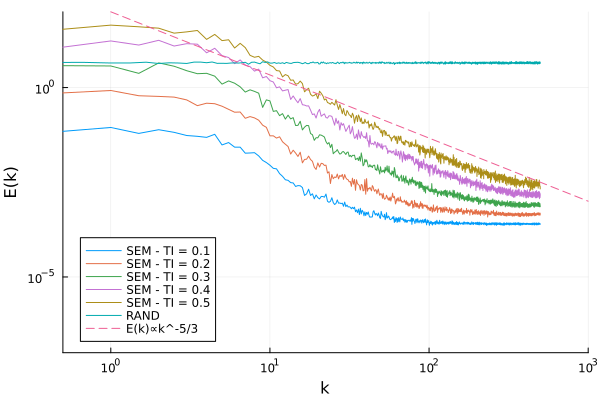
\includegraphics[width=0.45\textwidth]{Images/PSD/SEM_vs_RAND_tent.png}
         \caption{Power Spectral Density of the turbulent kinetic energy obtained using tent function}          
         \label{figsem:tentpsd}
\end{figure}

\begin{figure}[h]
         \centering
         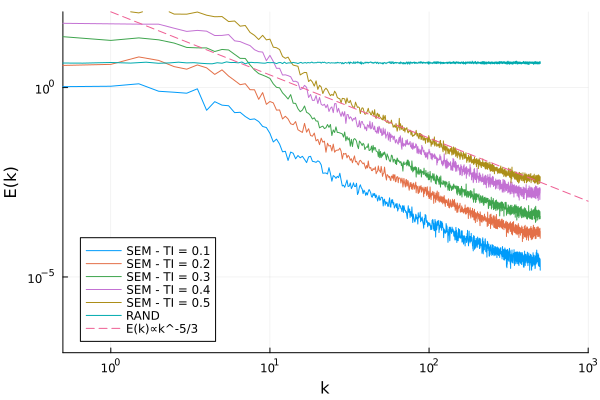
\includegraphics[width=0.45\textwidth]{Images/PSD/SEM_vs_RAND_step.png}
         \caption{Power Spectral Density of the turbulent kinetic energy obtained using step shape function}
            \label{figsem:steppsd}
\end{figure}


\begin{figure}[h]
         \centering
         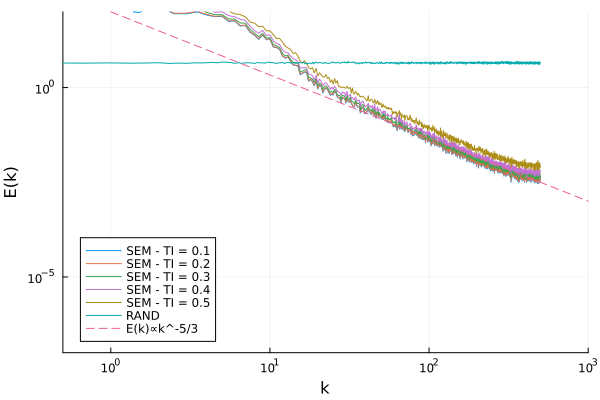
\includegraphics[width=0.45\textwidth]{Images/PSD/SEM_vs_RAND_gaus.png}
         \caption{Power Spectral Density of the turbulent kinetic energy obtained using gaussian shape function}
            \label{figsem:gauspsd}
\end{figure}






\begin{figure}[h]
     \centering          
     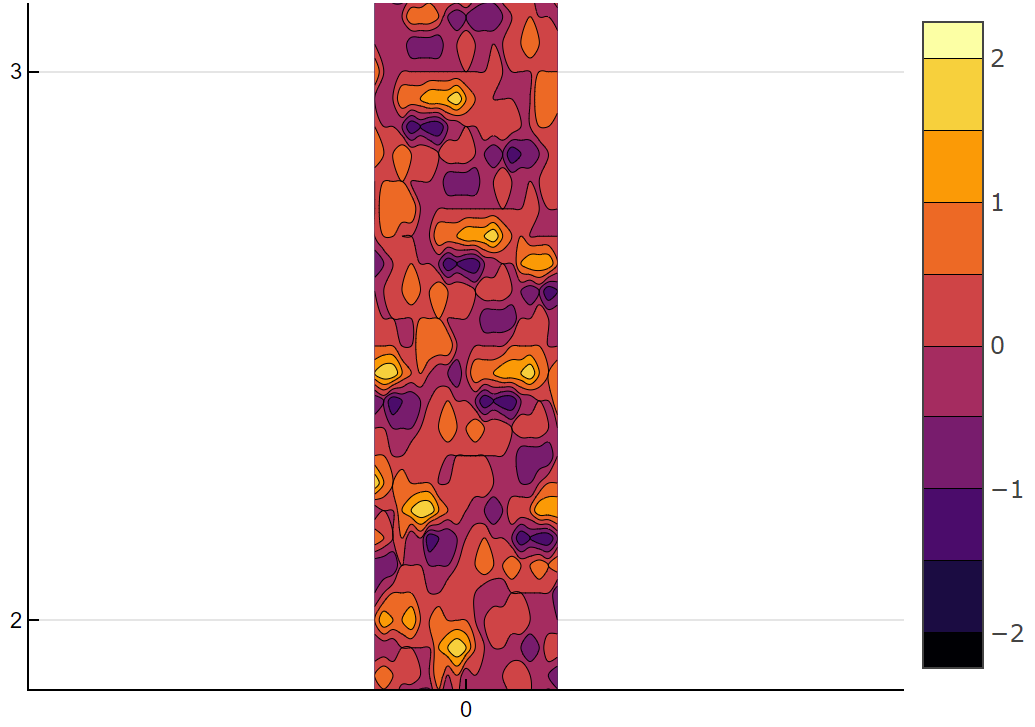
\includegraphics[width=0.45\textwidth]{Images/Eddy.png}
         \caption{Isovelocity contour on the XY plane for Z = 0}          
         \label{figsem:eddy_z0}
     \end{figure} 


\subsection{Divergence-free constraint}
Finally, it is fundamental to verify that all the effort put into implementing the DFSEM actually produces a divergence-free flowfield. 
Now, we are going to evaluate the fluctuations in 4 points useful for approximating the divergence using a simple forward derivative:
$$[x,y,z], [x+dx, y, z], [x,y+dy,z], [x,y,z+dz]$$

In order to verify the diverge-free condition is respected, the derivatives in each direction are computed with a simple forward method.
The divergence is normalized with the module of the gradient to obtain a non-dimensional quantity, \eqref{sem:norm_div}.
\begin{equation}
    \dfrac{\nabla\cdot \vec{u}}{|\nabla \vec{u}|}
    \label{sem:norm_div}
\end{equation}
Note: if $|\nabla \Vec{u}|$ is too small, it can lead to \texttt{NaN} values.

For the point at the centre of the domain the expression \eqref{sem:norm_div} is evaluated for $10e3$ time steps. The graph \ref{figsem:zero_div} shows that the DFSEM is actually creating a flow where the flow produces a divergence sufficiently close to zero. 

\begin{figure}[h]
     \centering          
     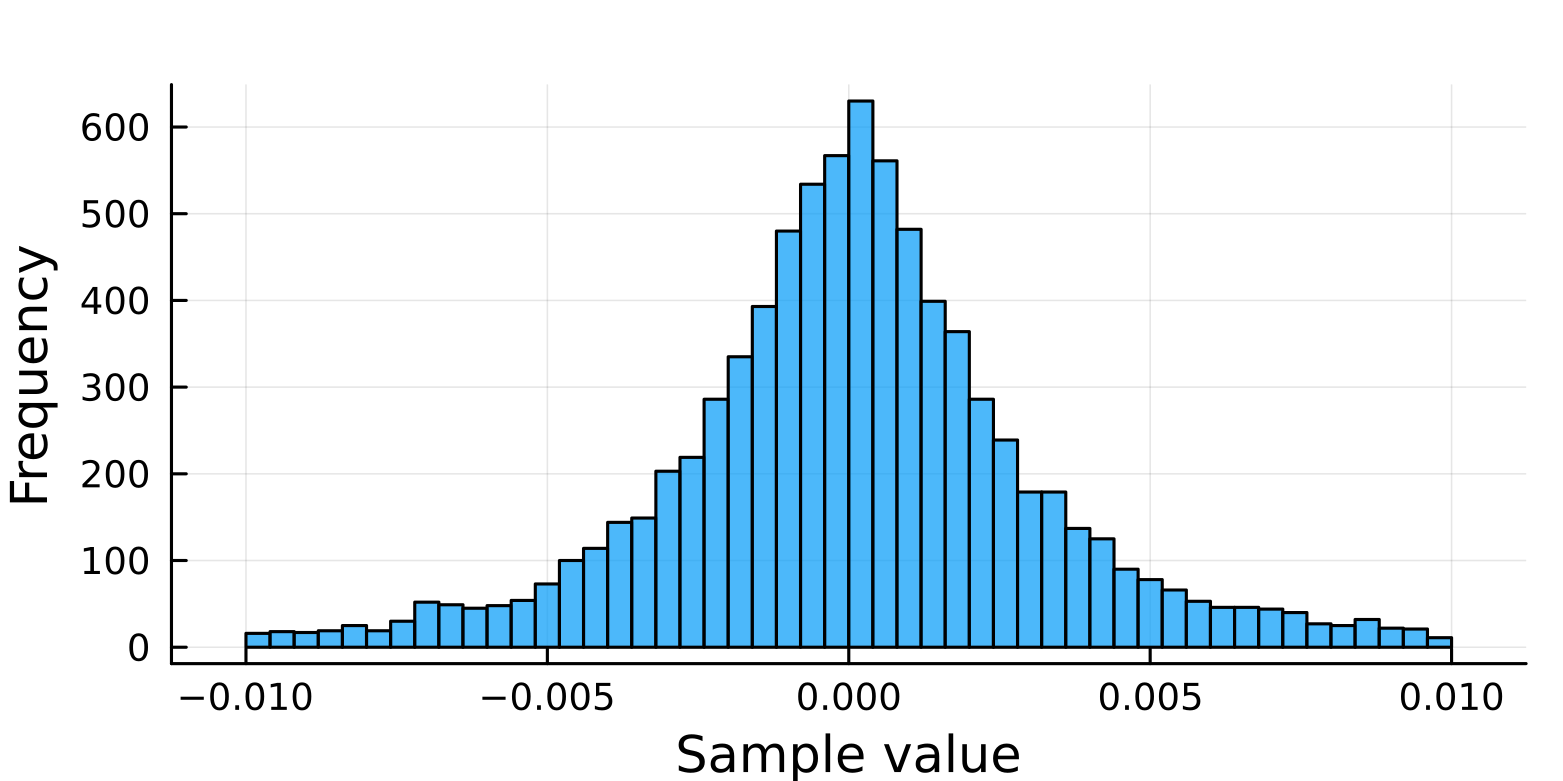
\includegraphics[width=0.45\textwidth]{Images/Statistics/dfsem_zero_div.png}
         \caption{Normalized divergence samples over 10000-time steps using DFSEM}          
         \label{figsem:zero_div}
\end{figure} 

Moreover, we analyze the normalized divergence at the plane X = 0, to confirm that it approaches zero almost everywhere in space. Figure \ref{figsem:zero_div_plane} illustrates how the derivative is almost zero everywhere, with only several local spots where the condition is not precisely fulfilled.

\begin{figure}[h]
     \centering          
     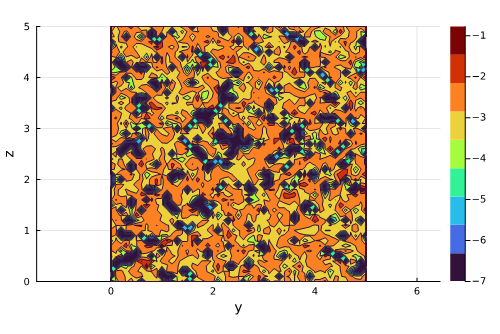
\includegraphics[width=0.45\textwidth]{Images/Statistics/Div_free_plane.pdf}
         \caption{Log10 of the absolute value of normalized divergence for plane X = 0 using DFSEM}          
         \label{figsem:zero_div_plane}
\end{figure} 

%\section{Aknoledgments}
% and \cite{simSEM}
 
 


% **************GENERATED FILE, DO NOT EDIT**************

\bibliographystyle{juliacon}
\bibliography{ref.bib}


\end{document}

% Inspired by the International Journal of Computer Applications template
